\section{Theory}

\subsection{Gamma Decay}

Alpha and beta decay usually give energy to the atomic core, which leads to excited nuclear staes.
Deexcitation of the core than leads to the emission of a high energetic photon, the gamma particle, with a specific energy.
These photons have an energy, depending on the core, in the range from $100$ kev to around $8$MeV.
The emission of the photon follows transition rules, depending on the Energy of the photon $E_{\gamma}$, angular momentum $L$ and the change of parity $\Delta \pi$.
Initial ($i$) and final ($f$) state have to follow the equation $E_{\gamma} = E_i - E_f$.
Depending on $L$ and $\Delta \pi$ we differentiate further between:
\begin{itemize}
\item $\Delta \pi (EL) = (-1)^L $ means electric multipole radiation ($EL$)
\item $\Delta \pi (EL) = (-1)^{L+1} $ means magnetic multipole radiation ($ML$)
\end{itemize}

\subsection{Interactions of Photons with Matter}

Photon interaction with matter is mainly dependant on the energy of the photons and the electric charge of the material it traverses.
In generel there are three interactions, which are:
\begin{itemize}
\item photoeffect
\item compton scattering
\item pairproduction
\end{itemize}
In the following section we will give a brief overview over these interactions.

\begin{figure}[ht]
	\centering
    \includegraphics[width=0.85\textwidth]{../plots/interactions.png}
	\caption{Dominating interactions of photons in matter}
	\label{interactions}
\end{figure}

\subsubsection{Photoeffect}

Photoeffect means the removal of electrons from the atomic shell, by absorbing a photon.
The energy of this electron van than be calculated as:
\begin{equation}
E = E_{\gamma} - U_B
\end{equation}
With the photon energy $E_{\gamma}$ and the binding energy of the material $U_B$.
In this experiment we will use a HPGe (high purity germanium) detector, where the photoeffect is dominated by the inner photelectric effect, where this happens inside a semiconductor.
In this case, an electron-hole-pair is created.
By applying a voltage on the detector, the electron and the hole are seperated and create a current, depending on the transfered energy.
In order for this to take place, the photon must have an energy higher than the binding energy of the material.
Because of this, we want detector material with a low binding energy for detectors with good resolution.
For example Ge has a binding energy of $U_B = \SI{0.67}{\electronvolt} $.
This is low enough, that we have to take thermal noise, created in the detector, into consideration, which means that we have to cool down the detector with liquid nitrogen.

Another detector we will use, is a scitnilator made of NaI.
Because of the lower charge of NaI, the outer photoelectric effect is dominating.
To detector this we use a photomultiplier (see Fig. \ref{theorie_PEV}).
Here we apply a voltage on the created photoelectrons, to target them on a dynode.
There they create new electrons and we apply again a voltage.
This is done a few times and we get a electric current, depending on the energy of the initial photon.

\begin{figure}[ht]
	\centering
    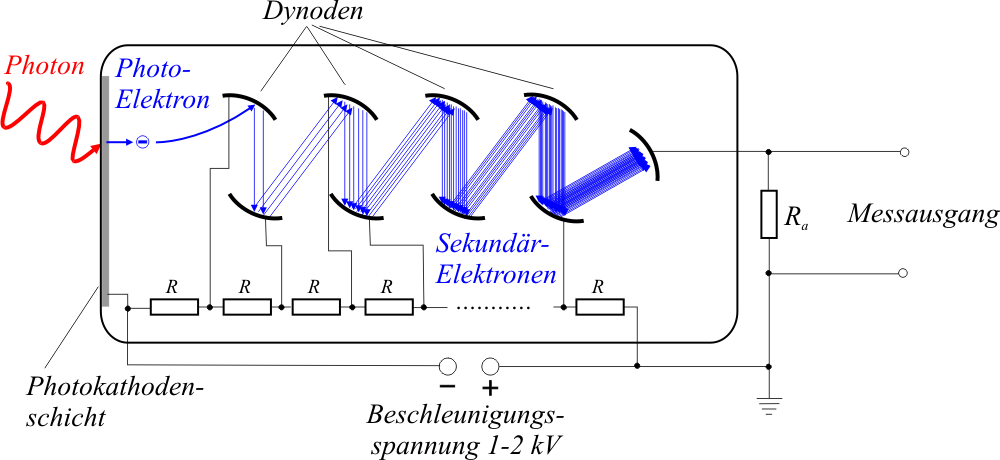
\includegraphics[width=0.85\textwidth]{../plots/Photomultiplier_schema_de.png}
	\caption{Photomultiplier \cite{Bild_Photomultiplier}}
	\label{theorie_PEV}
\end{figure}

Since the photoeffect leads to full transmission of the photonenergy, it leads to the creating of so called full energy peaks.
These are high peaks in the gamma spectrum of the detector.
By knowing the energy of gamma photons from the source, we can identify these peaks in the detector and find a curve, which shows the relatiion of detector channels and energy.
This is done during a detector calibration.

\subsubsection{Compton-Streuung}

Compton scattering is the eleastic scattering of a photon with a charged particle, usally an electron.
The energy of a photon scattered on an electron can be calculated as:
\begin{gather}
    E'_{\gamma}(\varphi) = \frac{E_{\gamma}}{1 + \frac{E_{\gamma}}{m_{e} c^{2}} (1 - \cos (\varphi))}
\end{gather}
With the scattered angle $\varphi$, (see Fig. \ref{theorie_Compton_Streuuung}), the initial energy of the poton $E_{\gamma}$ and the electron mass $m_e$

\begin{figure}[ht]
	\centering
    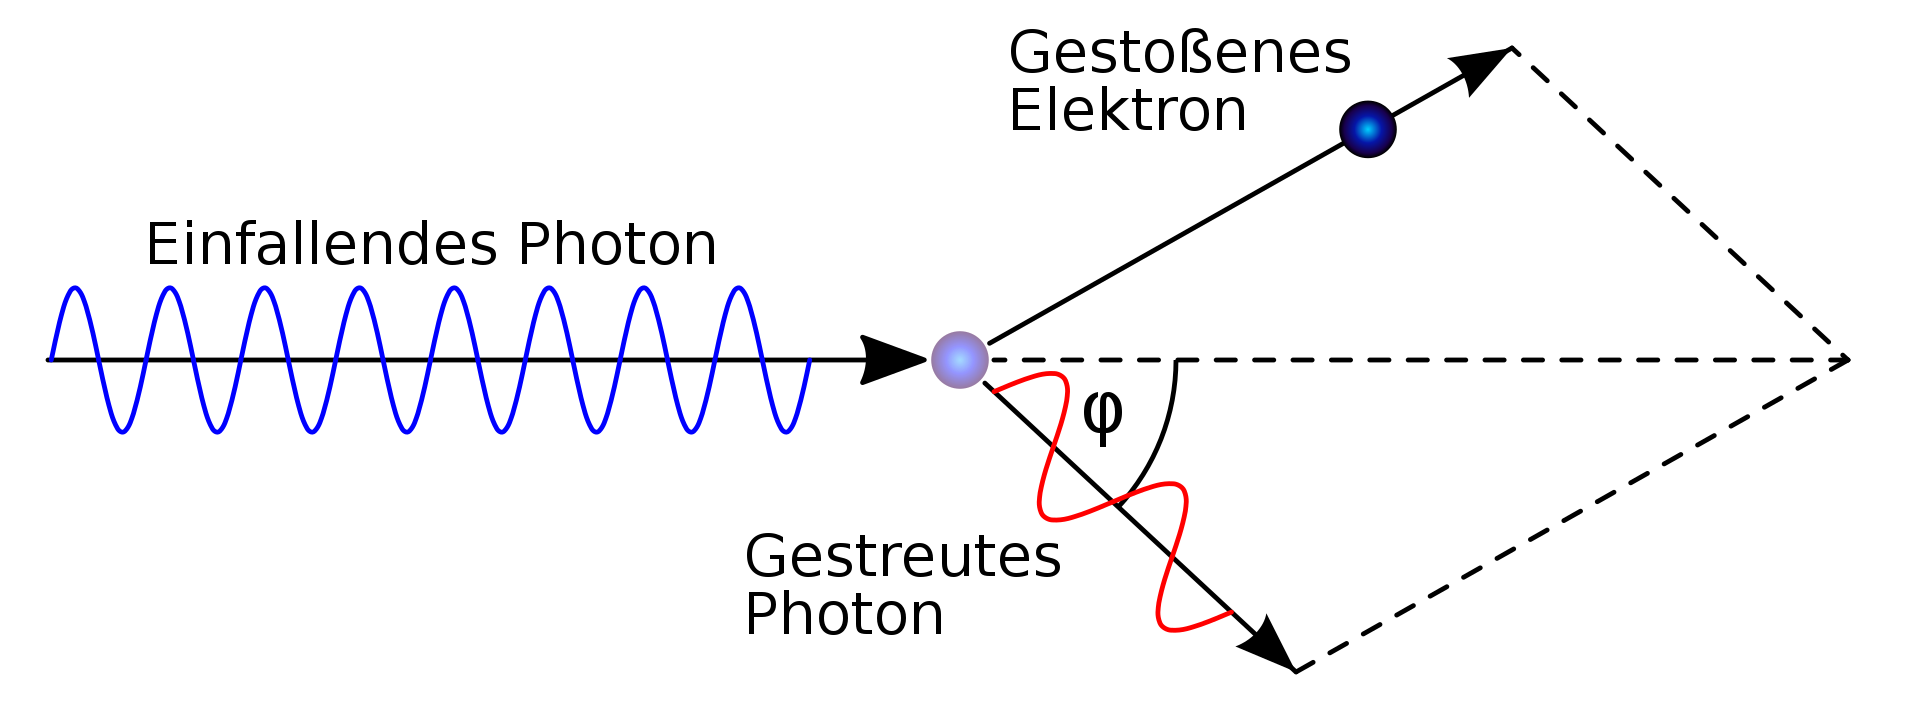
\includegraphics[width=0.85\textwidth]{../plots/The-geometry-of-Compton-scattering-showing-the-directions-of-the-scattered-photon-and.png}
	\caption{Schematic of compton scattering \cite{Bild_Compton_Streuung}}
	\label{theorie_Compton_Streuuung}
\end{figure}
Comtpon effect usually leads to 3 singificant structures in the detector spectrum:
\begin{itemize}
\item The angle depandance of the transmitted energy, leads to a continous amount of possible energies. In the spectrum, this is called the compton continuum.
\item Scattered particles with an angle of $180^{\circ}$ will gain maximum energy transmission. This creates a peak on the right edge of the comtpon continuum.
\item On the other edge of the continuum we get the backscatter peak, which comes from photons that are scattered backwards in the detector, before they can transmit all energy.
\end{itemize}

\subsubsection{Pairproduction}

Pair production is the creation of a particle-antiparticle-pair in the electric field of atomic shell or core.
For this process to happen, incoming photons need to have an energy of at least two times the mass of the created particle.
In the case of an electron positron pair, the photons need to have an energy of at least $2 \cdot m_e = 1022 \text{keV}$.
For all elements, pairproduction only dominates for energies above $5 \text{MeV}$ which is out of range of energies in this lab course.
